\documentclass[12pt,a4paper]{report}
\usepackage[utf8]{inputenc}
\usepackage[english]{babel}
\usepackage[T1]{fontenc}
\usepackage{amsmath}
\usepackage{amsfonts}
\usepackage{amssymb}
\usepackage{lmodern}
\usepackage{courier}
\usepackage[none]{hyphenat}
\usepackage{authoraftertitle}
\usepackage[final]{graphicx}
\DeclareGraphicsExtensions{.pdf,.png,.jpg}
\usepackage{geometry}
\geometry{a4paper, top=30mm, left=25mm, right=25mm, bottom=30mm,
	headsep=10mm, footskip=12mm}
\usepackage{color}
\usepackage{hyperref}
\usepackage[tikz]{bclogo}

\hypersetup{
	colorlinks=true,
	linkcolor=black,
	urlcolor=red,
	citecolor=black,
	linktoc=all
}

\usepackage{listings}
\definecolor{forestgreen}{RGB}{34,139,34}
\definecolor{orangered}{RGB}{239,134,64}
\definecolor{darkblue}{rgb}{0.0,0.0,0.6}
\definecolor{gray}{rgb}{0.4,0.4,0.4}

\lstdefinestyle{XML} {
	language=XML,
	extendedchars=true, 
	breaklines=true,
	breakatwhitespace=true,
	emph={},
	emphstyle=\color{red},
	basicstyle=\ttfamily,
	columns=fullflexible,
	commentstyle=\color{gray}\upshape,
	morestring=[b]",
	morecomment=[s]{<?}{?>},
	morecomment=[s][\color{forestgreen}]{<!--}{-->},
	keywordstyle=\color{orangered},
	stringstyle=\ttfamily\color{black}\normalfont,
	tagstyle=\color{darkblue}\bf,
	morekeywords={attribute,xmlns,version,type,release},
	otherkeywords={attribute=, xmlns=},
	basicstyle=\ttfamily\scriptsize
}


%Header & Footer
%\usepackage{lastpage}
%\rfoot{\thepage\ of \pageref{LastPage}}



\date{\today}
\author{Ari Ayvazyan}
\title{JEE Security Structure Part 1}

\begin{document}

\maketitle
\tableofcontents


\chapter{\MyTitle}
%\begin{flushright}
%        \MyAuthor, \MyDate
%\end{flushright}


\section{Introduction to Security Architecture}
Most web applications have a few things in common:\\
They need to figure out who is the user that is using the application and what is he allowed to do and see.\\\\
A typical application has more than one security layer, it may be protected by only being available from a specified network or VPN. In addition there usually is some kind of identity determination followed by a SQL user with permission to query only the required functions and data sets.\\
On top of this, there should be output escaping to ensure that a attacker, who is able to manipulate the output for other users, is limited in the harm he is able to cause.\\
\begin{figure}[h]
\centering
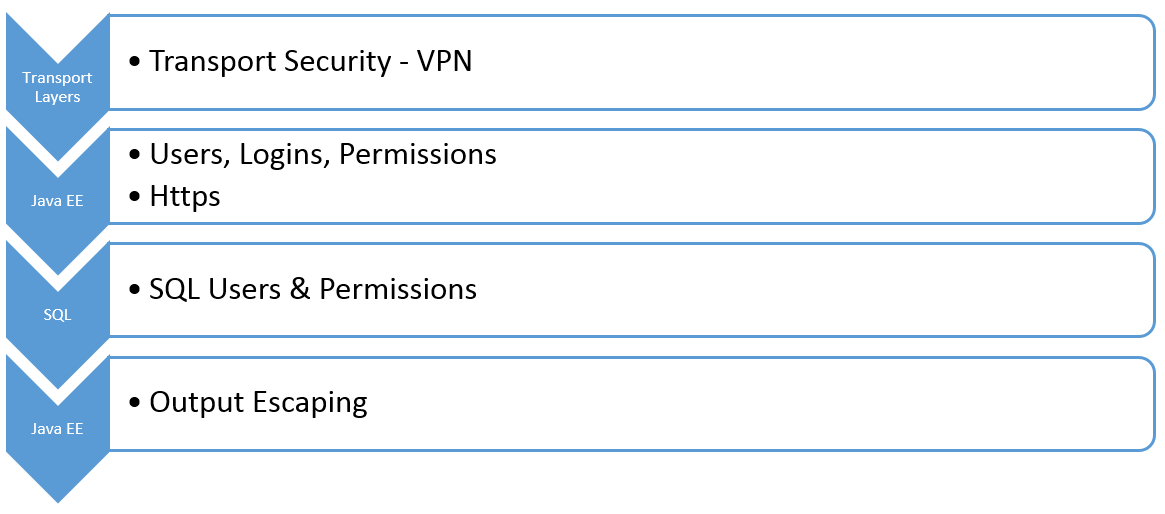
\includegraphics[width=1\linewidth]{res/SecurityLayers}
\caption{Security Layers in a common JEE application}
\label{fig:SecurityLayers}
\end{figure}
\newpage \noindent
According to Oracle\cite{oracleDoc}, there are two ways to implement such access control functionality with Java EE:
\begin{enumerate}
	\item Declarative Security (this includes Annotations and XML-Files)\\
	is applied during the application's deployment.
	\item Programmatic Security\\
	is applied by the application itself at runtime.
\end{enumerate}
While the programmatic implementation offers a wider range of customization, the declarative provides a well structured and easy to use approach.\\


\section{Authentication}
Authentication describes the identification process. This is mostly done by asking for a user-name \& password or sending a Token/Hash.

\section{Authorization}
Authorization is what happens after you are authenticated.\\
It deals with the question of what a authenticated person is allowed to do.\\
Authorization may be applied to URLs or resources like Beans and Servlets.\\

\begin{figure}[h]
	\centering
	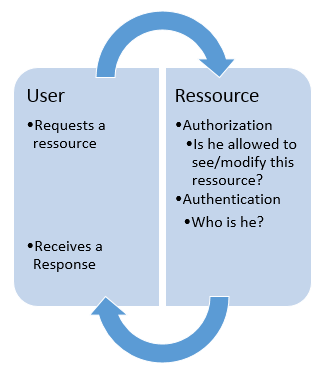
\includegraphics[width=0.5\linewidth]{res/AuthenAuthor}
	\caption{Authentication \& Authorization}
	\label{fig:AuthenAuthor}
\end{figure}

\section{Deployment Descriptors}
A Deployment Descriptor describes how a Java EE application should be deployed.\\
They contain information about security constraints, accessibility and resource references.\\\\
Deployment Descriptors are XML-Files that are by default located in the /WEB-INF/ directory.\\
The following deployment descriptors may be found here:
\begin{itemize}
	\item web.xml
	\item <vendor-specific>.xml (E.g. when using Glassfish: glassfish-web.xml)
\end{itemize}

\subsection{web.xml}
The Web.xml file stores apart from usual deployment information like servlet mappings also security related information about:\\
\begin{itemize}
	\item Protected Resources
	\item Security Roles
	\item Authentication methods
\end{itemize}
The following XML snippets are located within the <web-app></web-app> tag.
\newpage
\subsubsection*{Protected Resources}
It is possible to limit access to resources by defining a security constraint on the URL or by securing the resource itself.\\
E.g. to protect the /primes/ URL with all its subdirectories we would have to use the following code:\\
\begin{bclogo}[couleur=yellow!15,arrondi=0.1,logo=\bccrayon, ombre = true]{Securing a URL}
\begin{lstlisting}[style=XML]
<security-constraint>
	<web-resource-collection>
		<web-resource-name>primes
		</web-resource-name>
<!--Include /primes/ including all following subfolders-->
		<url-pattern>/primes/*</url-pattern>
<!-- This would result in a security leak because 
	there are more http-methods than GET and POST-->
<!-- by defining no http-method at all, 
	everything will be blocked-->
		<http-method>GET</http-method>
		<http-method>POST</http-method>
	</web-resource-collection>
	
	<auth-constraint>
		<role-name>view_role</role-name>
	</auth-constraint>
</security-constraint>
\end{lstlisting}
\end{bclogo}
In result, only a user with the role view\_role is allowed to access the defined resources.
\newpage
\subsubsection*{Security Roles}
A Security Role was used in the last subsection "Protected Resources", we declared that only users with the role "view\_role" are allowed to view the restricted URL.\\
A Security Role is a abstract layer in front of the container, it defines a identifier which we can use for constraints. This identifier is then used by the container to specify its meaning by telling who is part of this Security Role.\\
\begin{bclogo}[couleur=yellow!15,arrondi=0.1,logo=\bccrayon, ombre = true]{Defining a Security Role}
\begin{lstlisting}[style=XML]
    <security-role>
	    <description>This role has view access</description>
	    <role-name>view_role</role-name>
    </security-role>
\end{lstlisting}
\end{bclogo}
\subsubsection*{Authentication Methods}
There are several kinds of Authentication Methods with different security behaviors.\\
BASIC Authentication opens a login prompt when a user tries to access the secured URL, it is simple to implement but insecure. BASIC Authentication sends the user's credentials unencrypted to the server.\\
\begin{bclogo}[couleur=yellow!15,arrondi=0.1,logo=\bccrayon, ombre = true]{Defining BASIC Authentication}
\begin{lstlisting}[style=XML]
    <login-config>
	    <auth-method>BASIC</auth-method>
	    <realm-name>Java EE Login</realm-name>
    </login-config>
\end{lstlisting}
\end{bclogo}
\newpage
\subsection{(vendor-specific).xml}
Most containers use in addition to the web.xml a vendor specific XML file that is usually located in the same directory with web.xml.\\
E.g. Glassfish calls this file "glassfish-web.xml" while Tomcat has named it "context.xml".\\\\
The following settings can be configured there:\\
\begin{itemize}
	\item Principal – Role Mapping
	\item Group – Role Mapping
	\item Other container specific configuration.
\end{itemize}

\subsubsection{User Role Mapping}
It is possible to Map Users (Principals) to Roles. This setting is container dependent.\\
\begin{bclogo}[couleur=yellow!15,arrondi=0.1,logo=\bccrayon, ombre = true]{Principal mapping with Glassfish}
	\begin{lstlisting}[style=XML]
	<glassfish-web-app>
	<security-role-mapping>
		<role-name>view_role</role-name>
		<principal-name>Blitzmann</principal-name>
	</security-role-mapping>
	</glassfish-web-app>
	\end{lstlisting}
\end{bclogo}
This setting maps the user "Blitzmann" to the role "view\_role".
\newpage
\subsubsection{Group Role Mapping}
It is possible to Map Users (Principals) to Roles. This setting is container dependent.\\
\begin{bclogo}[couleur=yellow!15,arrondi=0.1,logo=\bccrayon, ombre = true]{Principal mapping with Glassfish}
	\begin{lstlisting}[style=XML]
	<glassfish-web-app>
	<security-role-mapping>
	<role-name>view_role</role-name>
	<group-name>view_group</group-name>
	</security-role-mapping>
	</glassfish-web-app>
	\end{lstlisting}
\end{bclogo}
This setting maps the group "view\_group" to the role "view\_role".
\section{Principals}
A Principal is a identity that can be authenticated.\\
E.g. a Unique user name\\
Principals are handled by the container and need to be configured there. This includes storage and queries\\

\section{Credential}
A Credential is defined as information that is used to authenticate a Principal.\\
E.g. a Password\\
Credentials are just like Principals handled by the container.

\section{Groups}
Groups and Principals can be mapped together. This information is handled by the container and by that not accessible by the application. To make this information available to the server, Groups can be mapped to Roles.\\
Group-Role mappings are usually defined in the (vendor-specific).xml file.\\

\section{Roles}
A Role is a abstract layer in front of the container that can be accessed application wide, they are declared in the web.xml file\\
Roles can be mapped to Principals and Groups via the (vendor-specific).xml file.\\

\section{Realms}
Realms are also known as Security policy domains, they store and provide information about Principals, their Credentials and their Groups.\\
A Realm may take use of a database, a file structure, a connection to a service...\\\\
Realms are handled by the container, some come with pre-configured realms.

\newpage
\section{Implementation Sample}
The following sample may be found at this URL:\\
\href{https://github.com/aayvazyan-tgm/JavaEESecurityExample}{https://github.com/aayvazyan-tgm/JavaEESecurityExample}\\
\subsection{Objective}
The objective of our sample is to deny access to our service, that is reachable at .../primes/, to everybody except users that are granted permission by possessing the "view\_role" role.
\begin{figure}[h!]
\centering
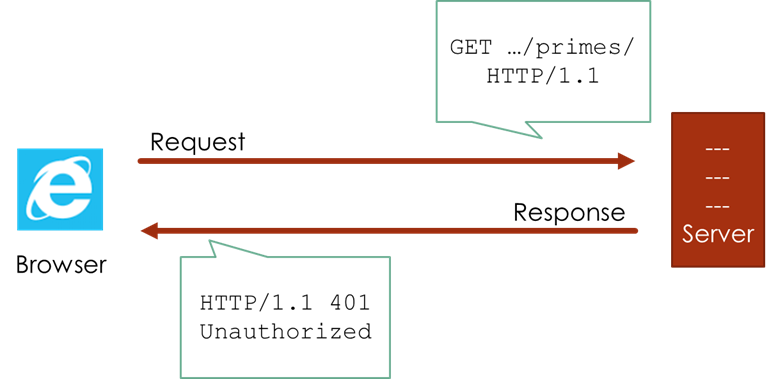
\includegraphics[width=1\linewidth]{res/Unauthorized}
\caption{The user tries to access a resource without authentication}
\label{fig:Unauthorized}
\end{figure}
\newpage \noindent
To figure out which user possesses the "view\_role" role, we first have to authenticate the user. This shall happen with a login promt. After transmitting the credentials to the server and having the correct role, the user should be able to access the resource.
\begin{figure}[h!]
	\centering
	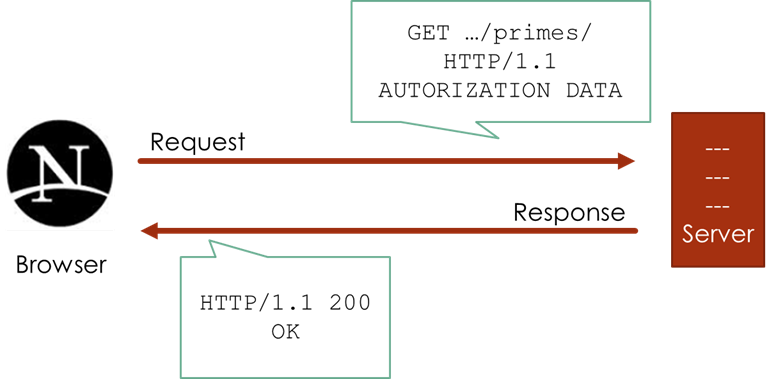
\includegraphics[width=1\linewidth]{res/Authorized}
	\caption{The user sends authentication data with his request}
	\label{fig:Authorized}
\end{figure}

\subsection{Setup}
A Glassfish server is used as the container.\\
The user "Blitzmann" was created by navigating to the GlassFish Server Administration Console, then to Configuration -> server-config -> Security -> Realms -> file -> add Property and entering "Blitzmann" as Name and the desired password as Value.\\
The rest is configured in the web.xml and glassfish-web.xml
\begin{bclogo}[couleur=yellow!15,arrondi=0.1,logo=\bccrayon, ombre = true]{web.xml}
	\begin{lstlisting}[style=XML]
    <security-constraint>
    <web-resource-collection>
	    <web-resource-name>primes</web-resource-name>
	    <!--Include all urls that are starting with /primes/ -->
	    <url-pattern>/primes/*</url-pattern>
	    <!-- This would result in a security leak because 
		    there are more http-methods than get and post-->
	    <!-- by defining no http-method at all 
		    everything will be blocked-->
	    <!--http-method>GET</http-method>
	    <http-method>POST</http-method-->
    </web-resource-collection>
	    <auth-constraint>
		    <role-name>view_role</role-name>
	    </auth-constraint>
    </security-constraint>
    
    <login-config>
	    <auth-method>BASIC</auth-method>
	    <realm-name>file</realm-name>
    </login-config>
    
    <security-role>
        <description>This role has view access</description>
        <role-name>view_role</role-name>
    </security-role>
	\end{lstlisting}
\end{bclogo}
\begin{bclogo}[couleur=yellow!15,arrondi=0.1,logo=\bccrayon, ombre = true]{glassfish-web.xml}
	\begin{lstlisting}[style=XML]
	<glassfish-web-app>
		<security-role-mapping>
			<role-name>view_role</role-name>
			<group-name>view_group</group-name>
			<principal-name>Blitzmann</principal-name>
		</security-role-mapping>
	</glassfish-web-app>
	\end{lstlisting}
\end{bclogo}
\section{Output Escaping}
Security vulnerabilities happen to be found in the best applications, it is important to have more layers of security that prevent attackers from reading or modifying sensitive information.\\
E.g. we have a guestbook, everybody is allowed to write a entry. To prevent a attacker from writing custom HTML into our site, we may use input escaping. But if the attacker has managed to someway access our database in a different way, where no input escaping is applied, he would be able to perform his attack on our users.\\
To prevent him from doing so, we have to check our output (Output Escaping). This means that we only allow data to be passed that makes sense, so we do not allow HTML elements in this case.\\
It is important to use a framework to do so, they are proven to work, tested and can even save working hours.

\section{Frameworks}
\subsection{Shiro}
Offers: Authentication, Authorization, Cryptography\\
Simple to use\\\\

\subsection{Spring}
Offers: Authentication, Authorization, Cryptography\\
Very structured\\\\

\subsection{JAAS - Java Authentication and Authorization Service}
Offers: Authentication, Authorization, Cryptography\\
Included in Java SE since Java 1.4 (javax.security.auth)\\\\

\section{Whats to come in Part 2 (Adrian)}
\begin{itemize}
	\item Working with Digital Certificates\\
	\item Securing Application Clients\\
	\item Security with Enterprise Beans\\
	\item Further Framework Information\\
\end{itemize}


\newpage
\begin{thebibliography}{99}
\bibitem{jSecVvulnerabilities}Java Security: Sicherheitslücken identifizieren und vermeiden, \\
Marc Schönefeld, 1. edition 2011\\
Publisher: Hüthig Jehle Rehm GmbH, Heidelberg. \\
ISBN/ISSN 978-3-8266-9105-8
\bibitem{EJSec}Enterprise Java Security: Building Secure J2EE Applications,\\
Marco Pistoia, Nataraj Nagaratnam, Larry Koved, Anthony Nadalin,\\
1. edition 2004 \\
Publisher: Addison-Wesley Professional.\\
ISBN/ISSN: ISBN 0-321-11889-8
\bibitem{oracleDoc}Official JavaEE Documentation, Oracle,\\
29.09.2014
http://docs.oracle.com/javaee/7/tutorial/partsecurity.htm\#GIJRP
Java EE 6,\\
Dirk Weil, 1. edition 2012\\
Publisher: entwickler.press\\
ISBN 978-3-86802-077-9
\bibitem{jeecookbook}Java EE 6 Cookbook for Securing, Tuning, and Extending Enterprise Applications,\\
Mick Knutson,\\
1. edition June 2012 \\
Publisher: Addison-Wesley Professional.\\
ISBN/ISSN: ISBN 9781849683166
\bibitem{JavaOne}JavaOne 2014: The Anatomy of a Secure Web Application Using Java, \\
Shawn McKinney \& John Field, September 29, 2014\\
San Francisco
\end{thebibliography}
\newpage
\listoffigures
\end{document}
